%Introduction and Motivations

Observing crawling ants how they manage to find a shortest path from a food source to their nest arises the question of how to model such a biological phenomena. It is known that the way ants organize their transporting system is based on a secreted chemical called pheromone. While ants move on a track they deposit a certain amount of pheromone. Since real ants prefer choosing lines of a high pheromone concentration, this messenger ensures that ants follow their members on a certain trail.
To illustrate the effect of pheromone on an ant trail consider Figure \ref{fig:ants}. Real ants follow a path between a food source and their nest (Fig. \ref{fig:ants} A). Placing an obstacle on the trail forces the ants to find a way of restoring the interrupted track (Fig. \ref{fig:ants} B). One expects half of the ants to turn right and half of them to turn left. In the beginning both ways around the obstacle are enriched with approximately the same amount of pheromone (Fig. \ref{fig:ants} C). Since ants that have chosen the shortest path need less time to pass by the obstacle the number of ants per time is bigger compared to those who have chosen the longer path. Consequently the shorter path contains a higher concentration of deposited pheromone than the longer one. This follows from the assumption that all ants secrete the same amount of pheromone and move approximately at the same speed. \\
After a certain time more ants prefer the shorter path containing more pheromone until the longer one is completely neglected to circumvent the obstacle (Fig. \ref{fig:ants} D).

\begin{SCfigure}[50]
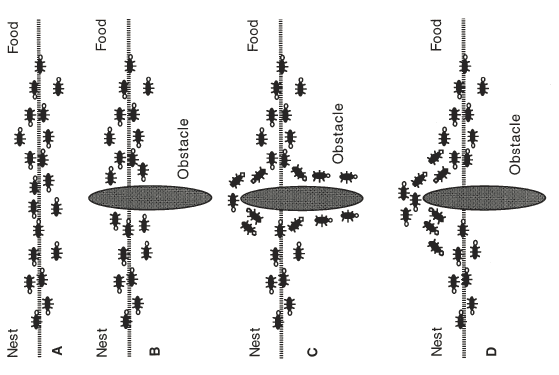
\includegraphics[width=0.5\linewidth]{ants}
\caption{(A): Ants following a trail between food source and their nest. (B): An obstacle is placed to interrupt the track of the ants. (C): The column of ants splits into two groups each choosing a different way to circumvent the obstacle. (D): Due to the higher concentration of pheromone all ants have chosen the shortest path.}
\label{fig:ants}
\end{SCfigure}

Consulting the literature \cite{paper} one finds an interesting paper which uses an ant colony system (ACS) to solve a traveling sales man problem (TSP). Artificial ants, also called agents are successively moving on a TSP graph between different cities. In the course of this they are following the constraint to visit each city once and return to their starting point. After all ants have completed their tour, the shortest one is rewarded by increasing the weight of the according tracks. This corresponds to a higher concentration of pheromone on the chosen tour.\\
The goal of this project is to implement the given model (see chapter \ref{sec:model} on page \pageref{sec:model}) from \cite{paper} and to calculate the shortest tour for different city environments. Those are obtained from the TSPLIB (\emph{http://www.iwr.uni-heidelberg.de/groups/comopt/software/TSPLIB95/tsp/}) and correspond to the data used in the reference paper \cite{paper}. The aim is to figure out whether our code is able to produce the same length of the shortest tour or not. Next to that, the variation of parameters in the model is analysed. Precisely, these simulations try to answer questions like: How does the shortest tour length depend on the rewarding, i.e. on the amount of pheromone deposited? How fast is the decay in the shortest tour as a function of completed rounds? Moreover, the influence of the number of agents on the time needed to find the shortest tour is investigated.